\section{Company Clustering Algorithm}

\subsection{Data}
To determine clusters of companies, its necessary to have a data-set that contains the relevant information
for a company, and has to be big enough to get meaningful results.

\begin{figure}[ht]
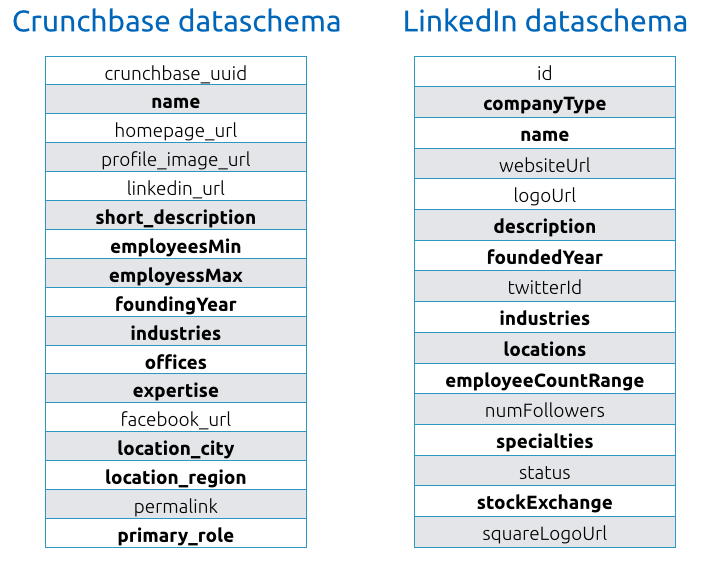
\includegraphics[scale=0.5]{sources_dataschema.png}
\centering
\caption{Comparison of dataschemas}
\label{fig:sourcesSchemas}
\end{figure}

\subsubsection{Datasources}
To ensure a good quality the data-sets were extracted from two different sources, LinkedIn and Crunchbase.

LinkedIn is a social business network with over 300 million user,\footnote{https://www.linkedin.com/about-us, 28th of June 2015} with people from all over the world. Apart
from user-profiles it also contains company-profiles with properties like year of foundation, industry or
number of employees. The information are maintained by the companies itself.

Crunchbase is an open database containing startup-activity and company information.\footnote{https://info.crunchbase.com/about/ 28th of June 2015} Company-datasets contain information
like employees, competitors, industry and basic information as well. Like the wikipedia information can be maintained by everyone,
which could lead to frequently updated information on the one hand, and to wrong information on the other hand.

Figure \ref{fig:sourcesSchemas} shows a subset of attributes of companies that are provided by each source. \footnote{More detailed information can be found on http://data.crunchbase.com/v3/docs/organization and https://developer.linkedin.com/docs/fields/company-profile }
The characteristics that represent information to conclude a companies demand are printed bold. \footnote{Regarding to influencing factors
and a companies environment in chapter 2 and 3. See also Chapter 4.3} Both datasets provide similar information but with a different structure.
For example the number of employees. Crunchbase provides 2 attributes one for the mininum value and one for the maximum value as integers
whereas LinkedIn delivers a string like ``1001-5000'' which requires further processing to extract the same information.

\begin{figure}[ht]
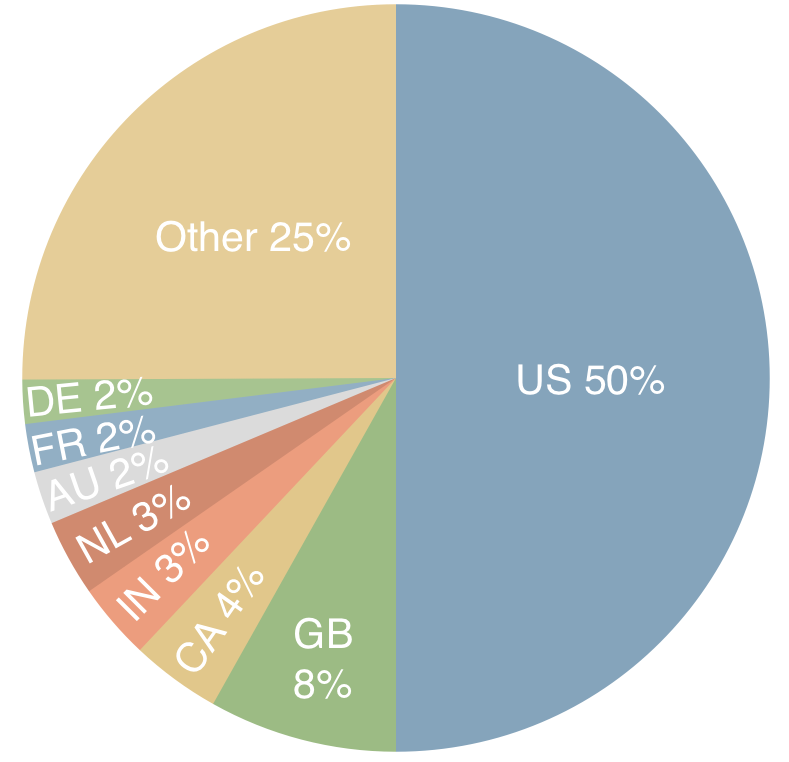
\includegraphics[scale=0.3]{companyCountries.png}
\centering
\caption{Distribution of companies per country (Total 236,235 companies)}
\label{fig:countryDistribution}
\end{figure}


\subsection{Dataprocessing}
Because both sources have different advantages and information and as mentioned in the last section a different structure,
it makes sense to combine both datasets into one, that covers all the necessary information needed for clustering,
and has one defined dataschema.

The biggest problem in combining these two datasets is finding the right corresponding company in the respectively
other dataset.
The used approach was to join to datasets on a 100\% match of both companynames. If companies have slightly different names
in both sets, they will be matched if they have the same website url given. Otherwise a new entry will be created in
the resulting dataset. This resulted in a dataset of 236,235 companies. As you can see in Figure \ref{fig:countryDistribution}
the most companies are located in the United States. The dataset contains companies from 220 countries.

[ Maybe add industries as well. ]




% Challenge: Finding a combination of Features which matches the closeness of companies
% to the need's development
\subsection{Company Features}
\label{companyFeatures}
Features are variables or a combination of variables that can describe certain characteristics of an entity. Using the right
features is essential to prove that strongly related businesses develop similar product needs. In this case the features have
to describe characteristics that influence a companies buying behaviour.

Regarding to Porter \cite{CompanyClusters} a company's \emph{location} has a high influence on how it acts. Companies will often rather know what happens next to
them than at a totally different place. Steps taken by companies right next to each other will have a higher impact on
how each of them reacts to particular circumstances, especially purchases made by one of the companies may lead to an economic
advantage. Other companies are then forced to close this gap by doing similar purchases.

Of course the location is important but has less impact if the companies next to each other do not compete somehow.
Referring to Porter \cite{CompanyClusters} companies of the same \emph{industry} are often shaped in clusters at one location.
They are using the same infrastructure and increasing the clusters know how.

So the first two features that cause the highest influence from one company to another are a company's location and its industry.

An increasing number of employees within a company leads to a higher complexity. Also bigger companies have other needs and higher expenses than
smaller ones have. Therefore companies of similar size are more related to each other than to smaller sized companies.
This leads us to the third feature, a company's size measured by its \emph{number of employees}.

According to Webster and Wind \cite{BusinessBuyingBehavior} companies are exposed to 6 different influences. These influences are already covered
by the selected features. For example by selecting a company's location the legal, economic and political influences which
are the strongest ones are considered.

Other characteristics mentioned in chapter 4.1 could also be used as features. But as the selected 3 features cover all the aspects
discussed during the economic background, there is no need for more features. A comparison of results using different combinations of
features could be part of future work. This thesis focuses on finding a correlation between the closeness of companies and their
demand-evolvement.

\subsection{Used Clustering Algorithm}

Some clustering approaches need to know the number of clusters. Of course one could estimate a number of clusters
by considering the number of industries as well as the number of different locations for each industry, but this would
still be an approximation to the number, which by the way would get invalid by adding more companies.
Hierarchical algorithms have the advantage that they do not need to know the number of used clusters. But this neither
solves the problem because one would still have to figure out which of the multiple generated clustering shemas
should be used.

Furthermore the used clustering algorithms has to be nonexclusive and intrinsic. It would not be on purpose to find
characteristics on predefined groups but rather to define groups of companies. An exclusive approach would provide
the information to which cluster a company belongs, not how close each of the companies are to each other.

So our approach has to be, to get an evaluation of all companies according to their closeness to each other. This
would also create some kind of clusters, but we would still have the information of closeness between each company.
An appropriate datastructure to store this information is a graph.

The aim to explore and furthermore predict the need evolvement could be achieved by having the additional
information of closeness between each company. To match the main thesis its important to find correlations between
closeness of companies and their needs.

Therefore the approach will be to calculate the proximity between each of the companies. This makes it possible to
look for existing correlations and still includes the oppotunity to create clusters for future work.

\subsection{Calculate Proximity}
The calculation is performed on a randomly sampled subset of our total set of companies to save time and keep the amount
of produced realations as small as possible. The subset contains 17737 documents. This would result in a maximum count of
realtionships of 157.291.716, where each company has a relationship to each other, but not itself. Thats the result of following
function where n equals the number of companies.

\begin{center}
  { \Large #relations \LARGE = $\frac{n*(n-1)}{2}$}
\end{center}

For the proximity we take all of the features and weight them according to their influence. According to the conclusions in chapter
\ref{companyFeatures} location and industry have a high weight whereas the company size does not have that much impact
on a company's buying behaviour. Therefor the first approach weights the location and industry 0.45 each and the size 0.1 times.

Show coverage of companies within cluster that match a product related demand. At the beginning , midtime and at the end.
Evaluate the goodness of the feature distribution by this development.

Showing that the clustering makes sense. Explain why its ok to ignore clusters that are only a company by itself. ->
To show the spreading over time within a cluster to show the well choseness of a cluster cant be shown with one company
cluster

{\small
\begin{tabular}{ccccccc}
  Clusters & Avg Rating & Level & High Avg & Big Cluster & Weight Sz In Lo & Tree depth \\
    5 & 0.7969 & 28 & 38\% & 1049 & 0,0,1 & 777 \\
    6 & 0.9860 & 67 & 22\% & 217 \(561\) &  1,0,0 & 284 \\
    6 & 0.9860 & 67 & 22\% & 217 \(561\) &  0,0,1 & 284 \\
    3 &
\end{tabular}
}
